\section{Feasibility and Scope}

\subsection{Target Audience}
\begin{frame}{Target Audience}
	The project aims to target the following audiences:
	\begin{enumerate}
		\item Law Enforcement Agencies: This includes local police departments and Federal Agencies.
		\item Private Security Firms: Companies specializing in security services
		\item Smart City Initiatives: City governments or organizations working on implementing smart city technologies for enhanced security
		\item Technology Providers for Law Enforcement: Companies developing and providing technology solutions for law enforcement purposes
		\item Government Security Agencies: Homeland Security, Border Patrol etc.
	\end{enumerate}
\end{frame}

\subsection{Feasibility}
\begin{frame}[allowframebreaks]{Feasibility}
	\begin{itemize}
		\item \textbf{Ethical and Legal Feasibility:}
			\begin{itemize}
				\item High-quality ethically-sourced datasets are publicly available for use.
				\item Data privacy and security can be ensured by collecting minimum data as per user consent.
			\end{itemize}
		\item \textbf{Technical Feasibility:}
			\begin{itemize}
				\item Over the decades, facial recognition technology has undergone significant advancements, with the integration of machine learning and deep learning models offering enhanced accuracy and efficiency. From classic computer vision techniques to contemporary deep learning architectures, the array of available methods showcases the feasibility of real-time facial recognition.
				\item Intermediary tasks can be handled using embeddings and feature extraction techniques.
				\item The seamless integration of detection, tracking, and recognition in real-time systems, especially those tailored for law enforcement scenarios, further accentuates the feasibility of deployment in dynamic environments.
			\end{itemize}
		\item \textbf{Scheduling Feasibility:} The project can be successfully completed within the term.
		
		\item \textbf{Economic Feasibility:}
			\begin{itemize}
				\item Model training can be done on consumer-grade hardware in addition to services like Google Colab, or LambdaCloud which provides low-cost Cloud GPUs:
				\begin{table}
					\vspace*{0.25cm}
					\centering
					\begin{tabular}{c|c|c|c|c}
						\textbf{VRAM (GB)} & 20 & 24 & 48 & 80 \\
						\hline
						\textbf{$\sim$INR/hr} & 30 & 35 & 63 & 166 \\
					\end{tabular}
					\vspace*{0.25cm}
				\end{table}
				\item Inference can be done on consumer-grade hardware without needing extra purchases.
			\end{itemize}

		\item \textbf{Operational Feasibility:} A user-friendly interface which accomplishes the objectives of the project with ease of maintenance and integration of future work can be developed.
	\end{itemize}
\end{frame}

\subsection{Scope}
\begin{frame}{Scope}
	The project has the following scope:
	\begin{enumerate}
		\item \textbf{Real-time Analysis:} Design and prototype a real-time face recognition system to operate in real-time, swiftly identifying faces even in dynamic and complex environments.
		
		\item \textbf{Crowded Settings:} One of the primary challenges the system aims to address is the identification of individual faces in densely populated areas, public gatherings, or bustling events.
		
		\item \textbf{Integration with Law Enforcement Databases:} The solution will be designed to seamlessly integrate with existing law enforcement databases, ensuring quick comparison and identification.
		
		\item \textbf{Robustness to Lighting and Environmental Conditions:} The system will be designed to work under varied lighting conditions, from well-lit environments to low-light or night-time settings.
	\end{enumerate}
\end{frame}

\subsection{Timeline Diagram}
\begin{frame}{Timeline Diagram}
	\centering
	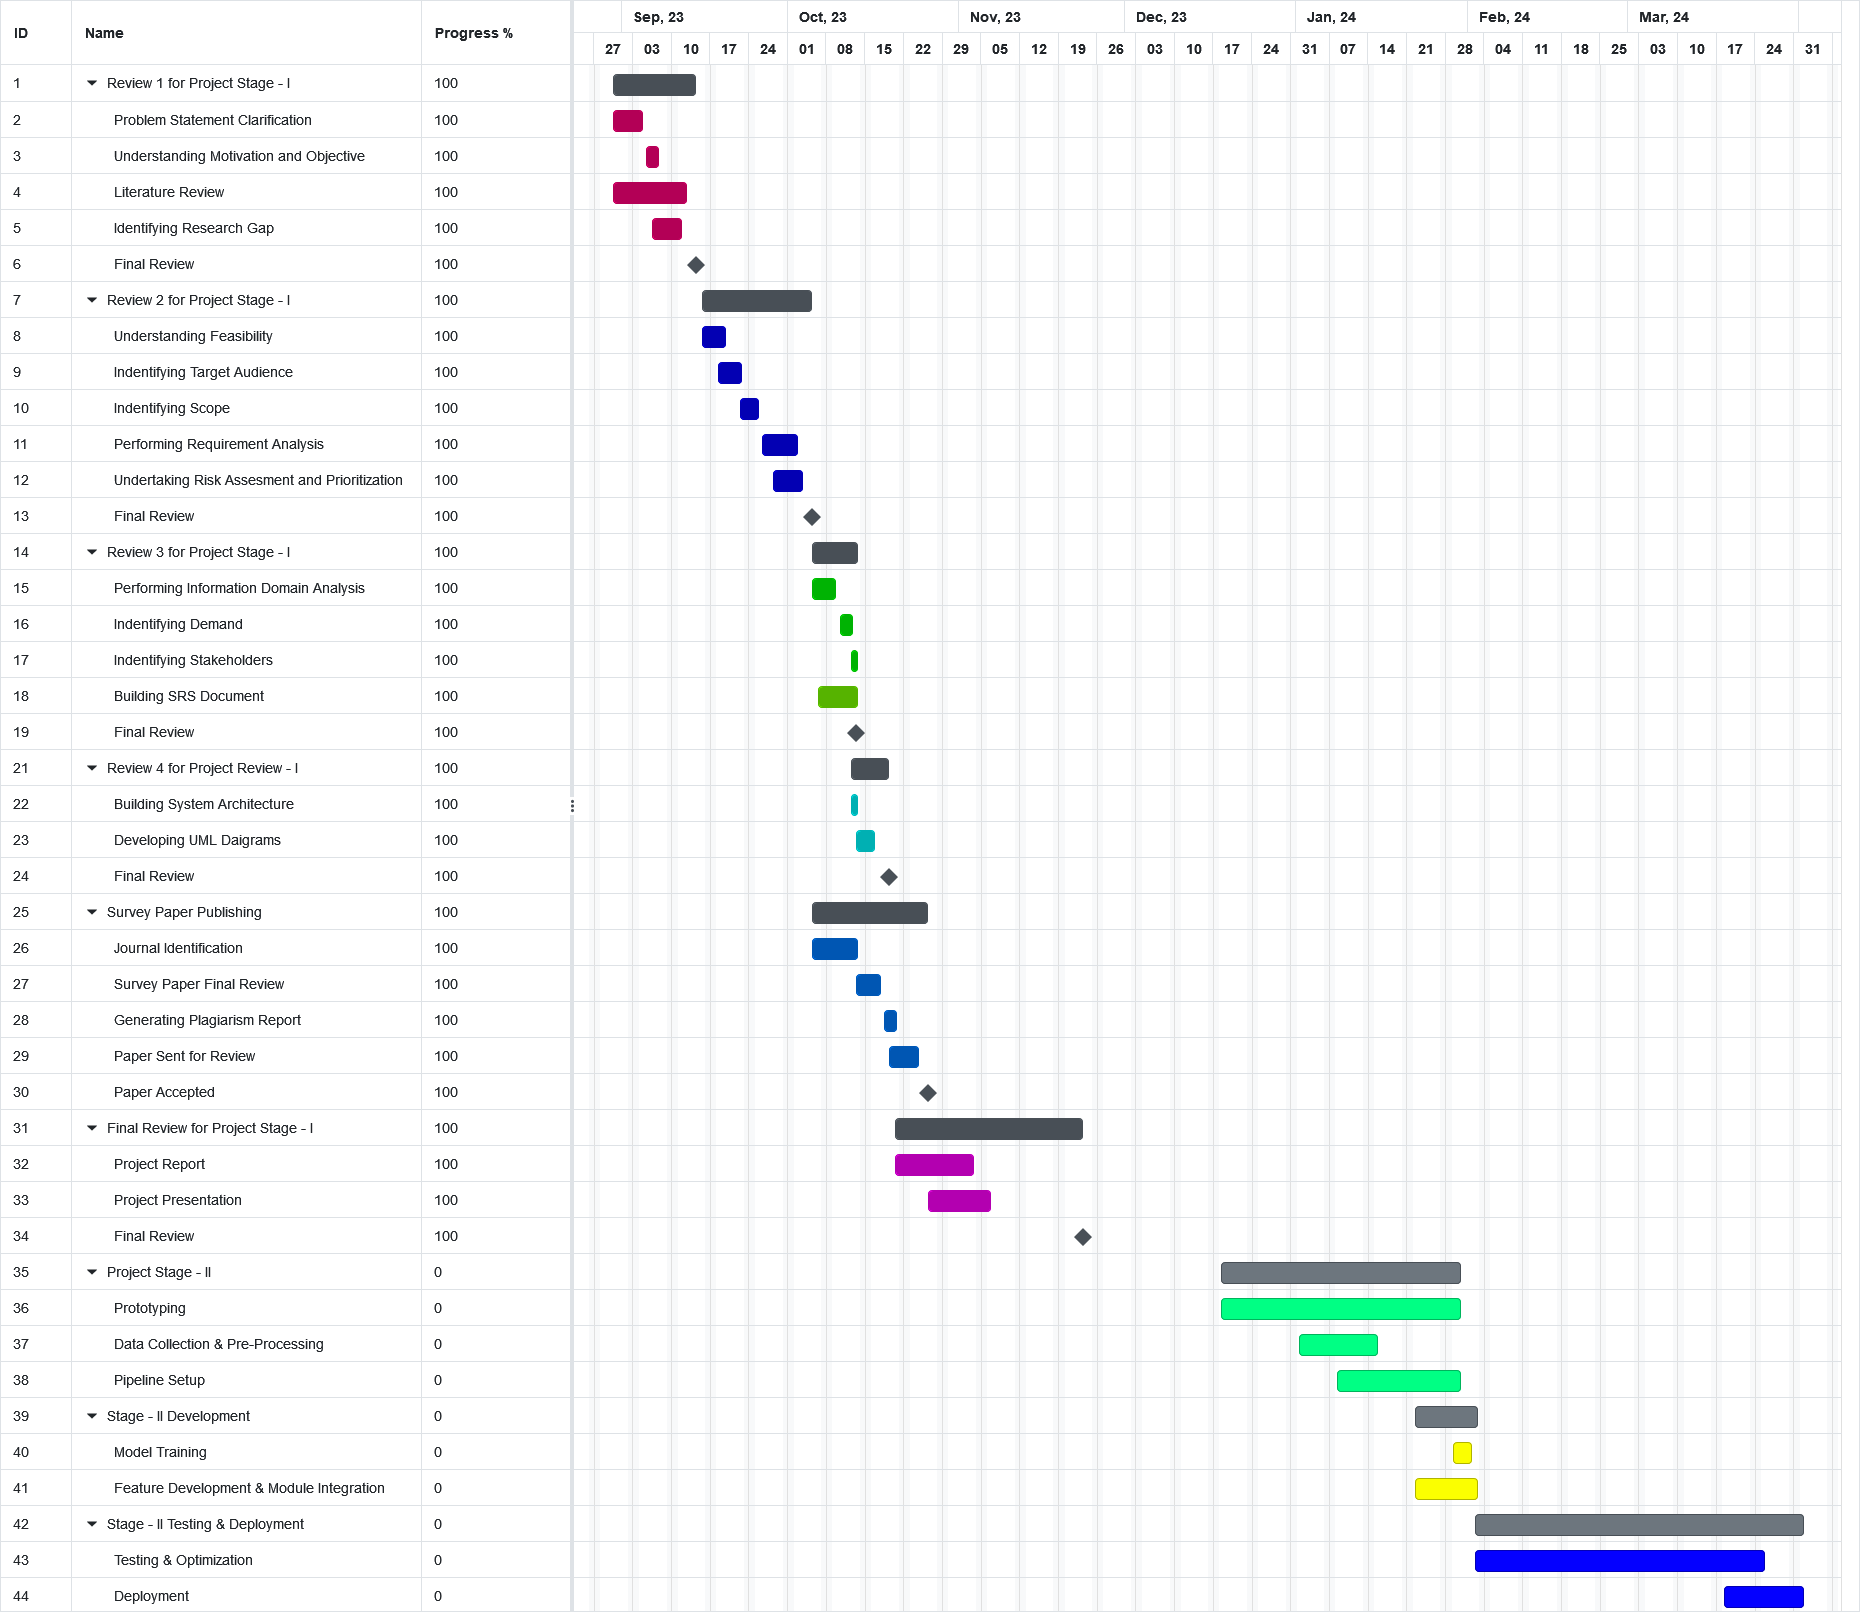
\includegraphics[height=0.8\textheight]{components/images/timeline.png}
\end{frame}

\subsection{Risk Assessment}
\begin{frame}{Risk Assessment}
	The following risks were identified with the project:
	\begin{enumerate}
		\item \textbf{Data Loss:} Losing facial data due to hardware failures or cyber-attacks. 
		\begin{itemize}
			\item This can be mitigated by regular backups, using RAID storage configurations, and ensuring strong cybersecurity measures.
		\end{itemize}

		\item \textbf{Environmental Challenges:} Factors like lighting, obstructions, and varying angles can affect the system's accuracy.
		\begin{itemize}
			\item This can be mitigated by use of algorithms that are robust to environmental changes and train the system with diverse environmental data.
		\end{itemize}

		\item \textbf{Adversarial Attacks:} Attackers might use methods like Master Faces to fool the recognition system.
		\begin{itemize}
			\item This can be mitigated by training the system to recognize and defend against adversarial inputs. Monitor for unusual activities.

		\end{itemize}
		
	\end{enumerate}
\end{frame}
